%------------------------------------------------------------------------------
%
% Repository path   : $HeadURL: https://hbergauer@forge.hephy.oeaw.ac.at/scm/svn/project-cmstrigger/GlobalTriggerUpgrade/doc/latex/gt-mp7-firmware-specification/content/framework.tex $
% Last committed    : $Revision: 4485 $
% Last changed by   : $Author: hbergauer $
% Last changed date : $Date: 2018-08-13 16:51:08 +0200 (Mon, 13 Aug 2018) $
% Description       : framework
% ------------------------------------------------------------------------------
\section{Framework}\label{sec:framework}
\textbf{Remark:}\\
with frame v1.2.3 "Delay Manager" (dm.vhd) and "Data Source Multiplexer" (dsmux.vhd) are removed because these features were never used in production system, only for tests.
Simmem data not useable anymore, because of removed dsmux.
The reason of removing is to get more available resources.\\

Figure \ref{fig_system_overview} shows the basic components the framework together with \rop. 
 
\begin{figure}[h]
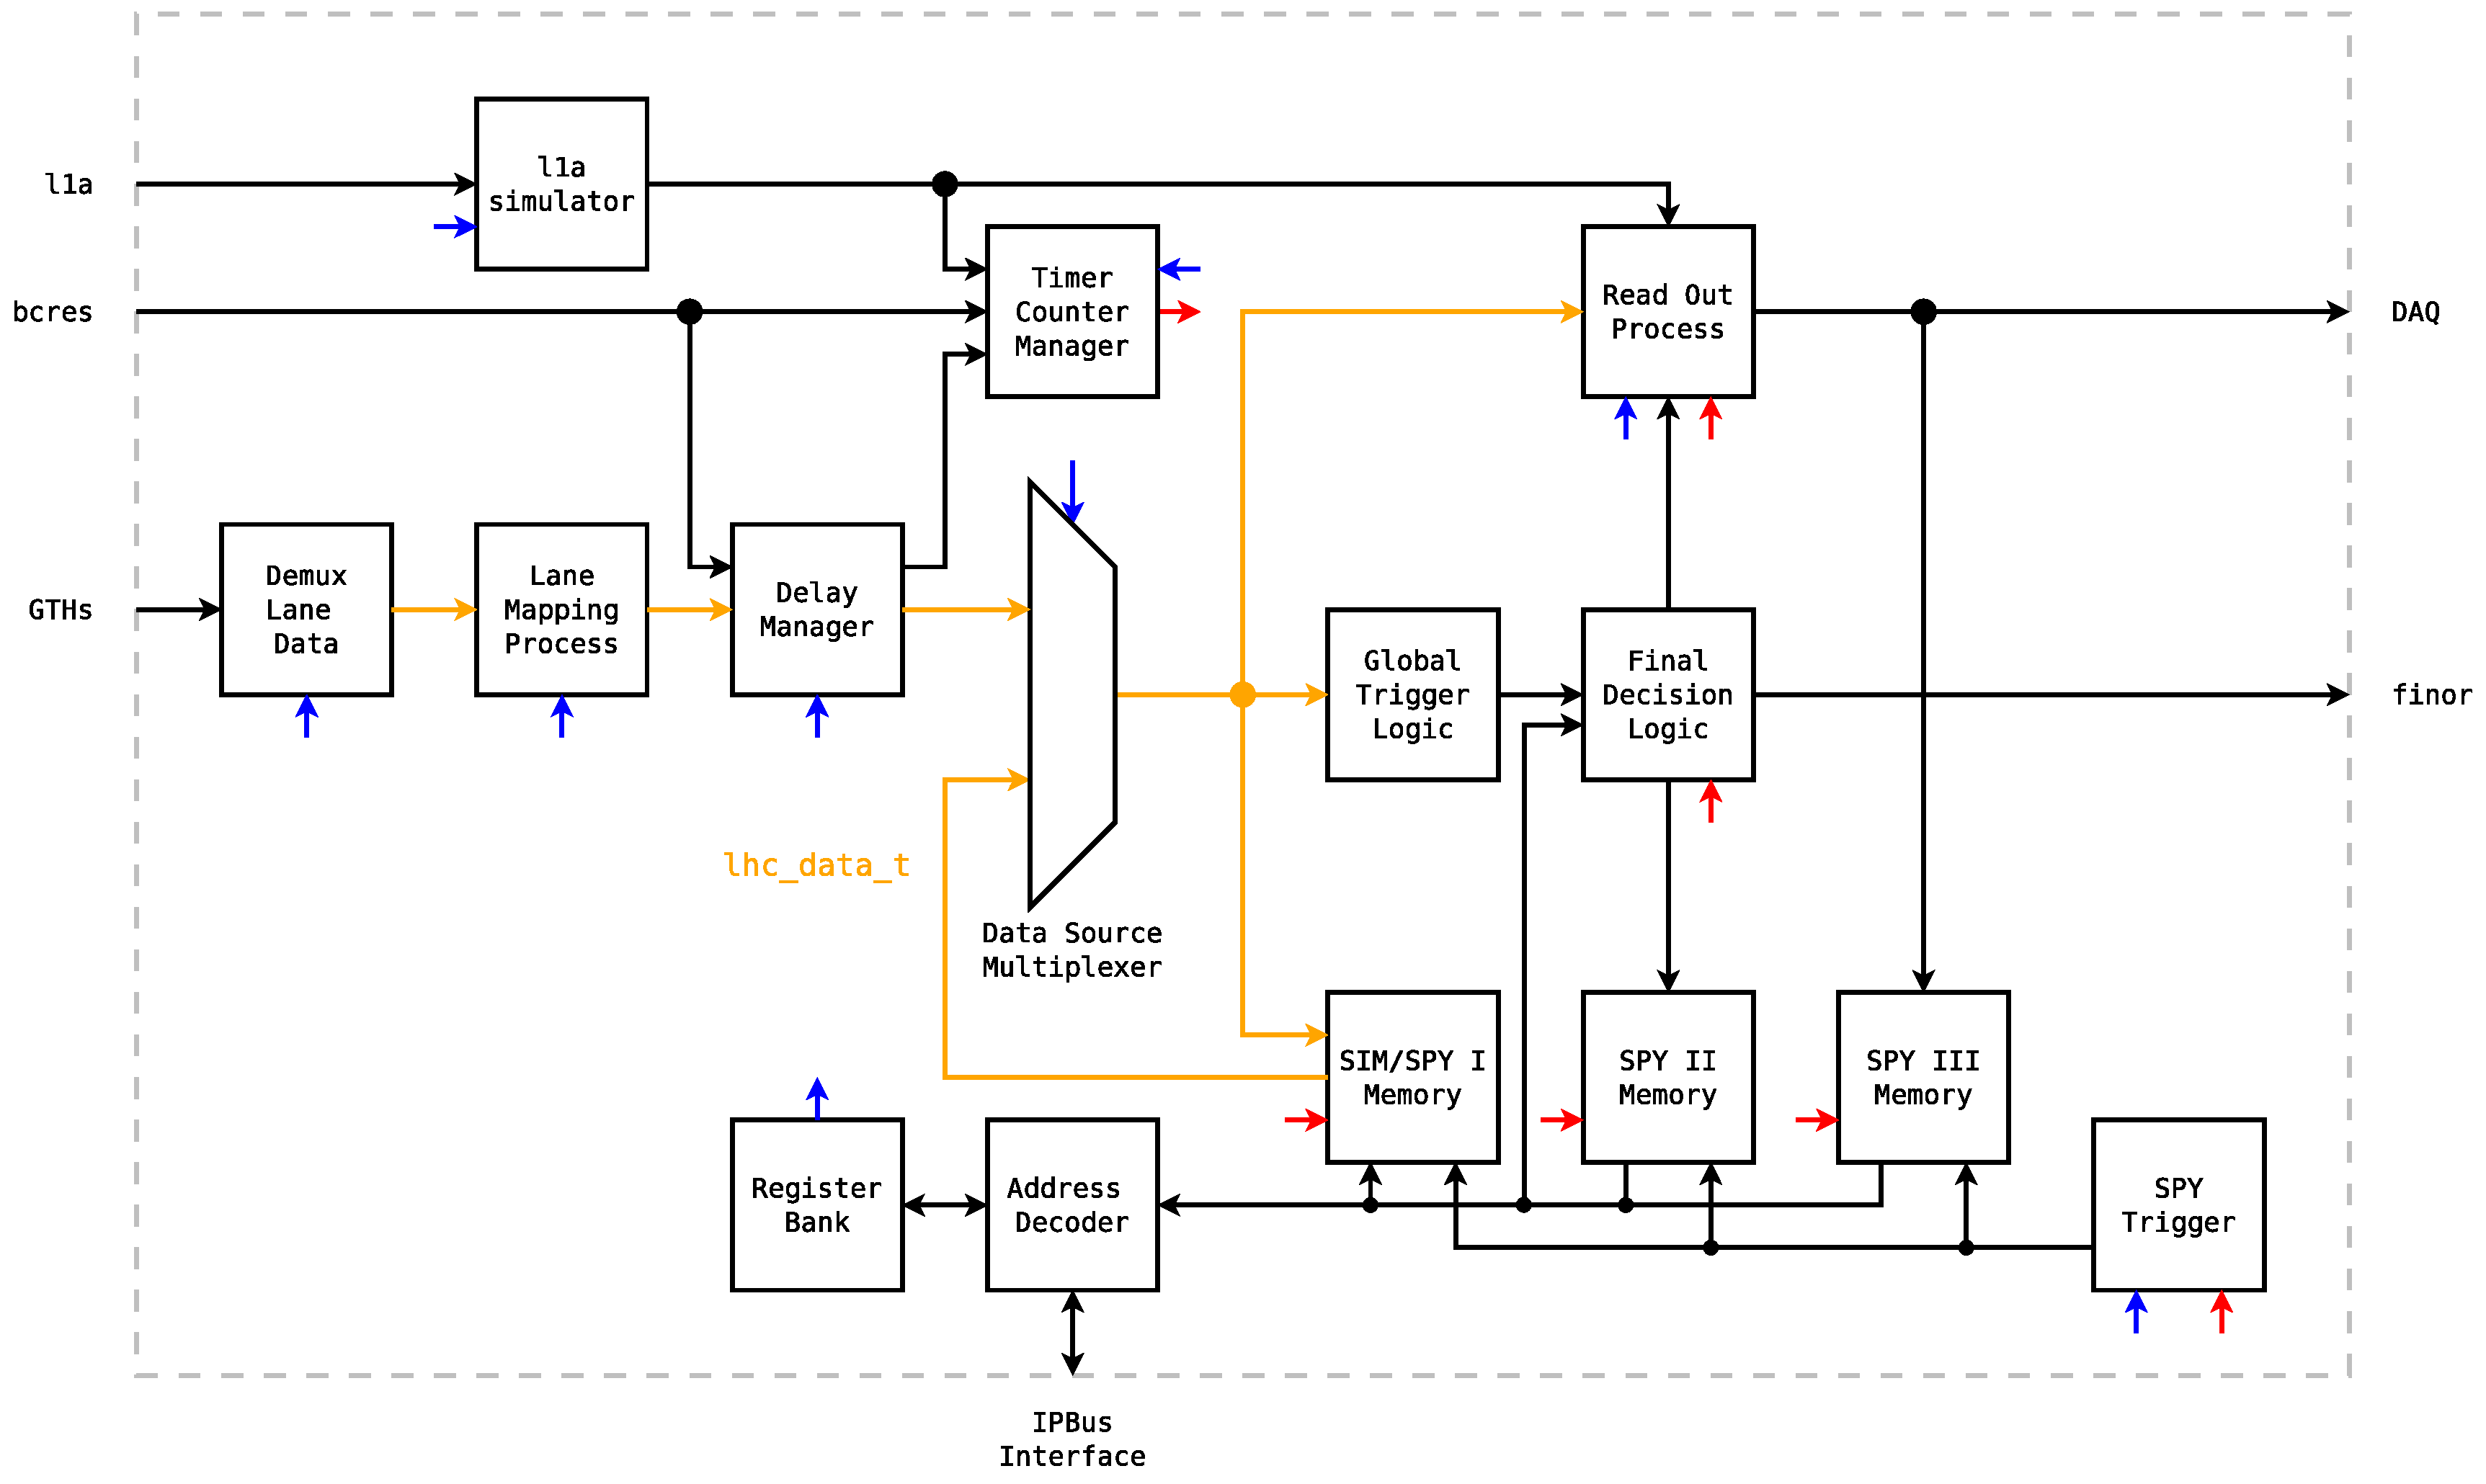
\includegraphics[width=1.0\textwidth]{./figures/system_overview}
\caption{System architecture overview}
\label{fig_system_overview}
\end{figure}

The central data type of the framework is shown in Listing \ref{lst_lhc_data_t} (see Section \ref{section_lhc_data_pkg} for details). In the current configuration it comprises 
2304 bits (288 Bytes). Data from the GTH interfaces is demultiplexed (from 240 MHz clock domain to LHC clock domain, see Demux Lane Data \ref{sec:demux_lane_data}) and mapped to this data type in the LMP (Lane Mapping Process). It is also used as input and output type for the SIM/SPY I memory. 
The DM (Delay Manager) takes the output of the LMP and applies software configurable delays to the the different object streams (e.g. muon data, jet, tau etc.) in the \texttt{lhc\_data\_t} 
to produce a consistent output (also regarding to the bcres signal). The software configurable multiplexer DSMUX (Data Source Multiplexer) is used to select which data stream is used as 
input for the processing elements (trigger logic). The output of the DSMUX is routed to the GTL (Global Trigger Logic) and ROP (Read Out Process) and can optionally be stored in the SPY I memory.

\subsection{Configuration of optical connections} \label{sec:sec_configuration_optical_conn}
The configuration of the optical connections to Calo-Layer2 is (currently) done as described in Table~\ref{tab:framework:tab_configuration_optical_conn}, where
frame means the 32 bits data (240 MHz) within a LHC clock period. 

% \begin{table}[htdp]
% \vspace{5mm}
% \begin{center}
% \begin{tabular}{|c|m{.13\columnwidth}|m{.13\columnwidth}|m{.13\columnwidth}|m{.13\columnwidth}|m{.13\columnwidth}|m{.13\columnwidth}|}
% % \begin{tabular}{|p{.04\columnwidth}|p{.13\columnwidth}|p{.13\columnwidth}|p{.13\columnwidth}|p{.13\columnwidth}|p{.13\columnwidth}|p{.13\columnwidth}|}\hline
% % \begin{tabular}{|c|c|c|c|c|c|c|}\hline
% % \textbf{lane nr} & \textbf{1\textsuperscript{st}} & \textbf{2\textsuperscript{nd}} & \textbf{3\textsuperscript{rd}} & \textbf{4\textsuperscript{th}} & \textbf{5\textsuperscript{th}} & \textbf{6\textsuperscript{th}} \\\hline\hline
% \cline{2-7}
% & \multicolumn{6}{ c| }{\textbf{frame}} \\\hline
% % \textbf{link} & \makebox [.13\columnwidth][c]{\textbf{frame}} & \makebox [.13\columnwidth][c]{\textbf{frame}} & \makebox [.13\columnwidth][c]{\textbf{frame}} & \makebox [.13\columnwidth][c]{\textbf{frame}} & \makebox [.13\columnwidth][c]{\textbf{frame}} & \makebox [.13\columnwidth][c]{\textbf{frame}} \\
% \textbf{link} & \makebox [.13\columnwidth][c]{\textbf{0}} & \makebox [.13\columnwidth][c]{\textbf{1}} & \makebox [.13\columnwidth][c]{\textbf{2}} & \makebox [.13\columnwidth][c]{\textbf{3}} & \makebox [.13\columnwidth][c]{\textbf{4}} &\makebox [.13\columnwidth][c]{\textbf{5}} \\\hline\hline
% 0 & reserved & reserved & muon obj. 0 [0..31] & muon obj. 0 [32..63] & muon obj. 1 [0..31] & muon obj. 1 [32..63]\\\hline
% 1 & reserved & reserved & muon obj. 2 [0..31] & muon obj. 2 [32..63] & muon obj. 3 [0..31] & muon obj. 3 [32..63]\\\hline
% 2 & reserved & reserved & muon obj. 4 [0..31] & muon obj. 4 [32..63] & muon obj. 5 [0..31] & muon obj. 5 [32..63]\\\hline
% 3 & reserved & reserved & muon obj. 6 [0..31] & muon obj. 6 [32..63] & muon obj. 7 [0..31] & muon obj. 7 [32..63]\\\hline
% 4 & \egamma obj. 0 & \egamma obj. 1 & \egamma obj. 2 & \egamma obj. 3 & \egamma obj. 4 & \egamma obj. 5 \\\hline
% 5 & \egamma obj. 6 & \egamma obj. 7 & \egamma obj. 8 & \egamma obj. 9 & \egamma obj. 10 & \egamma obj. 11 \\\hline
% 6 & jet obj. 0 & jet obj. 1 & jet obj. 2 & jet obj. 3 & jet obj. 4 & jet obj. 5 \\\hline
% 7 & jet obj. 6 & jet obj. 7 & jet obj. 8 & jet obj. 9 & jet obj. 10 & jet obj. 11 \\\hline
% 8 & tau obj. 0 & tau obj. 1 & tau obj. 2 & tau obj. 3 & tau obj. 4 & tau obj. 5 \\\hline
% 9 & tau obj. 6 & tau obj. 7 & tau obj. 8 & tau obj. 9 & tau obj. 10 & tau obj. 11 \\\hline
% 10 & \ett, ETTEM, MBT0HFP & \htt, TOWERCOUNT, MBT0HFM & \etm, MBT1HFP & \htm, MBT1HFM & \etm\_HF & \htm\_HF (preliminary definition) \\\hline
% 11 & free & free & free & free & free & free \\\hline
% 12 & external-conditions [0..31] & external-conditions [32..63] & reserved & reserved & reserved & reserved \\\hline
% 13 & external-conditions [64..95] & external-conditions [96..127] & reserved & reserved & reserved & reserved \\\hline
% 14 & external-conditions [128..159] & external-conditions [160..191] & reserved & reserved & reserved & reserved \\\hline
% 15 & external-conditions [192..223] & external-conditions [224..255] & reserved & reserved & reserved & reserved \\\hline
% \end{tabular}
% \end{center}
% \caption{Configuration of optical connections}
% \label{tab:framework:tab_configuration_optical_conn}
% \end{table}

\begin{table}[htdp]
\vspace{5mm}
\begin{center}
\begin{tabular}{c|m{.13\columnwidth}|m{.13\columnwidth}|m{.13\columnwidth}|m{.13\columnwidth}|m{.13\columnwidth}|m{.13\columnwidth}|}
\cline{2-7}
 & \multicolumn{6}{c|}{\textbf{frame}} \\\hline
\multicolumn{1}{|c|}{\textbf{link}} & \makebox[.13\columnwidth][c]{\textbf{0}} & \makebox[.13\columnwidth][c]{\textbf{1}} & \makebox[.13\columnwidth][c]{\textbf{2}} & \makebox[.13\columnwidth][c]{\textbf{3}} & \makebox[.13\columnwidth][c]{\textbf{4}} &\makebox[.13\columnwidth][c]{\textbf{5}} \\\hline\hline
\multicolumn{1}{|c|}{0} & reserved & reserved & muon obj. 0 [0..31] & muon obj. 0 [32..63] & muon obj. 1 [0..31] & muon obj. 1 [32..63]\\\hline
\multicolumn{1}{|c|}{1} & reserved & reserved & muon obj. 2 [0..31] & muon obj. 2 [32..63] & muon obj. 3 [0..31] & muon obj. 3 [32..63]\\\hline
\multicolumn{1}{|c|}{2} & reserved & reserved & muon obj. 4 [0..31] & muon obj. 4 [32..63] & muon obj. 5 [0..31] & muon obj. 5 [32..63]\\\hline
\multicolumn{1}{|c|}{3} & reserved & reserved & muon obj. 6 [0..31] & muon obj. 6 [32..63] & muon obj. 7 [0..31] & muon obj. 7 [32..63]\\\hline
\multicolumn{1}{|c|}{4} & \egamma obj. 0 & \egamma obj. 1 & \egamma obj. 2 & \egamma obj. 3 & \egamma obj. 4 & \egamma obj. 5 \\\hline
\multicolumn{1}{|c|}{5} & \egamma obj. 6 & \egamma obj. 7 & \egamma obj. 8 & \egamma obj. 9 & \egamma obj. 10 & \egamma obj. 11 \\\hline
\multicolumn{1}{|c|}{6} & jet obj. 0 & jet obj. 1 & jet obj. 2 & jet obj. 3 & jet obj. 4 & jet obj. 5 \\\hline
\multicolumn{1}{|c|}{7} & jet obj. 6 & jet obj. 7 & jet obj. 8 & jet obj. 9 & jet obj. 10 & jet obj. 11 \\\hline
\multicolumn{1}{|c|}{8} & tau obj. 0 & tau obj. 1 & tau obj. 2 & tau obj. 3 & tau obj. 4 & tau obj. 5 \\\hline
\multicolumn{1}{|c|}{9} & tau obj. 6 & tau obj. 7 & tau obj. 8 & tau obj. 9 & tau obj. 10 & tau obj. 11 \\\hline
\multicolumn{1}{|c|}{\multirow{3}{*}{10}} & 
\multicolumn{1}{l|}{\ett} & \htt & \etm & \htm & ET$_{miss}^{HF}$ & HT$_{miss}^{HF}$ \\
\multicolumn{1}{|c|}{} &
\multicolumn{1}{l|}{ETTEM} & TOWER-COUNT & ASYMET & ASYMHT & ASYM-ETHF & ASYM-HTHF \\
\multicolumn{1}{|c|}{} &
\multicolumn{1}{l|}{MBT0HFP} & MBT0HFM & MBT1HFP & MBT1HFM & CENT[3:0] & CENT[7:4] \\\hline
\multicolumn{1}{|c|}{11} & free & free & free & free & free & free \\\hline
\multicolumn{1}{|c|}{12} & external-conditions [0..31] & external-conditions [32..63] & reserved & reserved & reserved & reserved \\\hline
\multicolumn{1}{|c|}{13} & external-conditions [64..95] & external-conditions [96..127] & reserved & reserved & reserved & reserved \\\hline
\multicolumn{1}{|c|}{14} & external-conditions [128..159] & external-conditions [160..191] & reserved & reserved & reserved & reserved \\\hline
\multicolumn{1}{|c|}{15} & external-conditions [192..223] & external-conditions [224..255] & reserved & reserved & reserved & reserved \\\hline
\end{tabular}
\end{center}
\caption{Configuration of optical connections}
\label{tab:framework:tab_configuration_optical_conn}
\end{table}

%------------------------------------------------------------------------------
%
%  Demux Lane data
%
% ------------------------------------------------------------------------------

\subsection{Demux Lane Data} \label{sec:demux_lane_data}
Data from GTH interfaces is in the 240 MHz clock domain. The demultiplexing to the LHC clock domain (about 40 MHz) is done in demux\_lane\_data.vhd, which is instantiated
in frame.vhd as often as lanes are used (currently 16 lanes are used). 

%------------------------------------------------------------------------------
%
%  Lane Mapping Process
%
% ------------------------------------------------------------------------------

\subsection{Lane Mapping Process} \label{sec:lmp}
In the Lane Mapping Process module data from the lanes are mapped to objects structure defined in lhc\_data\_pkg.vhd.

\subsubsection{Implementation}\label{sec:lmp_impl}
Currently lane mapping is "fixed" in lmp.vhd module, see Table \ref{tab:framework:current_lane_mapping}

\begin{table}[htdp]
\vspace{5mm}
\begin{center}
\begin{tabular}{|c|l|c|}\hline
\textbf{lane} & \textbf{objects} \\\hline\hline
0 & muon objects 0..1 \\\hline
1 & muon objects 2..3 \\\hline
2 & muon objects 4..5 \\\hline
3 & muon objects 6..7 \\\hline
4 & \egamma objects 0..5 \\\hline
5 & \egamma objects 6..11 \\\hline
6 & jet object 0..5 \\\hline
7 & jet object 6..11 \\\hline
8 & tau object 0..5 \\\hline
9 & tau object 6..11 \\\hline
10 & \esums (incl. minimum bias trigger bits and towercounts) \\\hline
11 & n/a (currently not used) \\\hline
12 & external-conditions [0..63] \\\hline
13 & external-conditions [64..127] \\\hline
14 & external-conditions [128..191] \\\hline
15 & external-conditions [192..255] \\\hline
\end{tabular}
\end{center}
\caption{Current lane mapping}
\label{tab:framework:current_lane_mapping}
\end{table}

%------------------------------------------------------------------------------
%
%  Delay Manager
%
% ------------------------------------------------------------------------------

\subsection{Delay Manager} \label{sec:dm}
\textbf{Remark:}\\
with frame v1.2.3 "Delay Manager" (dm.vhd) and "Data Source Multiplexer" (dsmux.vhd) is removed because these features were never used in production system, only for tests.
The reason of removing is to get more available resources.\\

The Delay Manager is responsible for creating a delayed version of the \texttt{lhc\_data} and the bcres signal on its input. 
For this purpose it uses an internal memory to record the history of the input signals.

\subsubsection{Implementation}\label{sec:dm-impl}
The DM is basically a reimplementation of the concept of the last design. The reimplementation was necessary because the new framework version uses the register bank for 
software registers and the old DM was not flexible enough to handle the \texttt{lhc\_data\_t} introduced in the new framework.

The DM instantiates one \texttt{delay\_element} for every object type defined in the \texttt{lhc\_data\_t} (e.g. muon, eg, etc.). The \texttt{delay\_element} uses RAM blocks 
to implement the delay line. However, for the delays 0 and 1 this memory can not be used (write latency) and must be bypassed (Figure \ref{fig_dm_delay_element}).

\begin{figure}[h]
\begin{center}
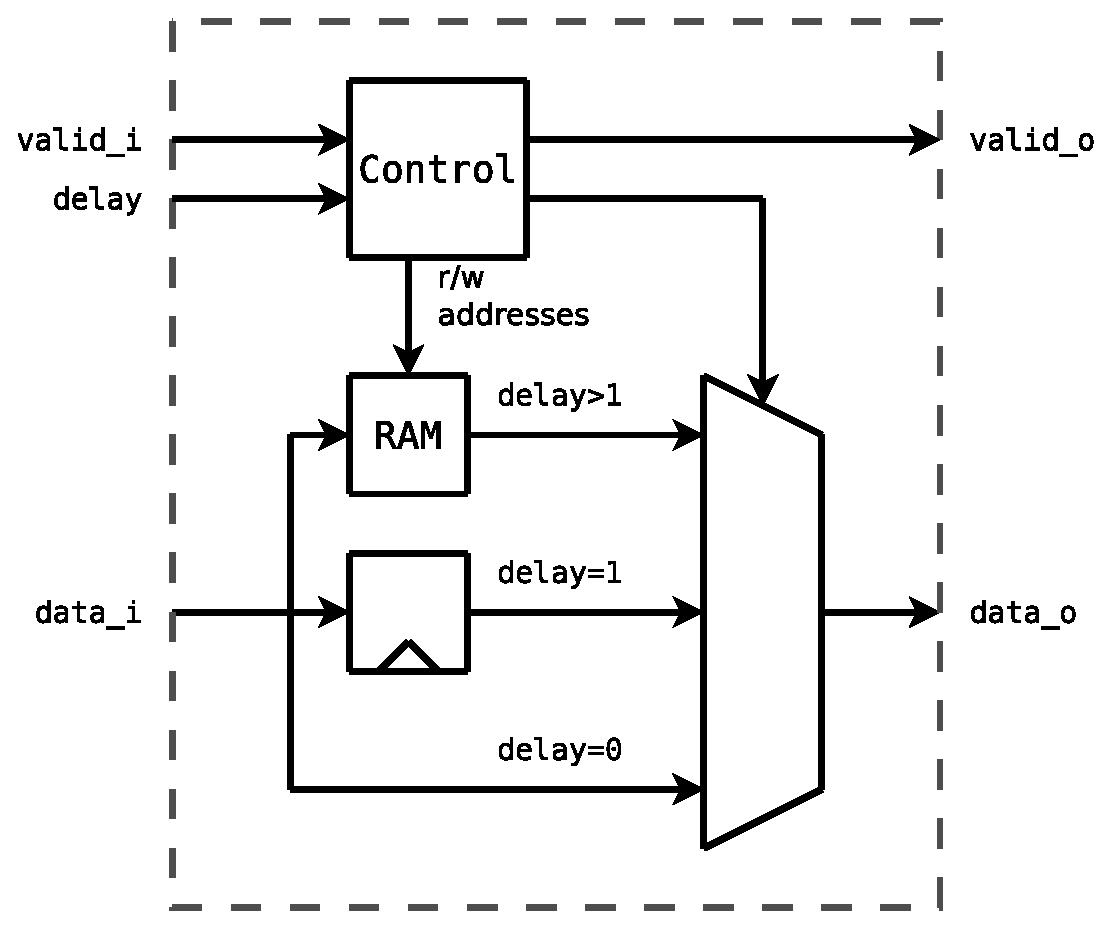
\includegraphics[width=0.5\textwidth]{./figures/dm_delay_element}
\end{center}
\caption{Delay Manager: delay\_element}
\label{fig_dm_delay_element}
\end{figure}

The Implementation of the DM is very generic because it makes extensive use of the constants provided by the \texttt{lhc\_data\_pkg}. The $lhc\_data\_i$ input signal 
is converted into a \texttt{std\_logic\_vector}.
The constants \texttt{LHC\_DATA\_SLV\_START\_INDICES} and \texttt{LHC\_DATA\_SLV\_OBJECT\_WIDTH} provide the start index of each object in this vector and their 
width respectively. The number of objects is given by the \texttt{LHC\_DATA\_OBJECT\_COUNT} constant. This information is used by a for-generate statement to instantiate 
the required \texttt{delay\_element} components.

For the $bcres\_o$ and the $bcres\_FDL\_o$ signals two additional \texttt{delay\_element} components are instantiated. 

If only the data width or the array size of an object in the \texttt{lhc\_data\_t} is changed the DM does not need any modification. If, however, a new object is added a 
new delay register must be added, as described in the register bank section. 

The registers for all delays have the same layout (see Register \ref{dm_reg}). The names for the individual (per object) delay registers are given in Table \ref{tab_dm_regs}. 
For the software addresses of these registers refer to the \texttt{xml/gt\_amc514\_dm.xml} file.

\begin{register}{htbp}{Delay Manager Registers}{}% name=CONFIG
	\label{dm_reg}
	\regfield{reserved}{20}{12}{0}%
	\regfield{delay}{12}{0}{0}%
	\begin{regdesc}
	\begin{reglist}[Request~Depth]
		\item [delay] The delay in lhc clock cycles (40 MHz) used for the specific object data.
	\end{reglist}
	\end{regdesc}
\end{register}

\begin{table}[h]
\vspace{5mm}
\begin{center}
\begin{tabular}{|c|c|}
\hline
object description & register name \\ \hline  \hline
bcres for TCM & bcres\_tcm\_delay \\ \hline
bcres for FDL & bcres\_fdl\_delay  \\ \hline
muon data & muons\_delay  \\ \hline
e/g & eg\_delay  \\ \hline
tau & tau\_delay \\ \hline
jet & jet\_delay  \\ \hline
ett & ett\_delay  \\ \hline
ht & ht\_delay  \\ \hline
etm & etm\_delay  \\ \hline
htm & htm\_delay  \\ \hline
external conditions & ex\_con\_delay  \\ \hline
\end{tabular}
\end{center}
\caption{delay manager registers}
\label{tab_dm_regs}
\end{table}

% \subsubsection{Interface Specification}\label{sec:dm-inter}
% \begin{minipage}{\textwidth}
% \lstinputlisting[language=VHDL,caption=DM interface specification]{interfaces/dm.vhd}
% \end{minipage}
% 
%------------------------------------------------------------------------------
%
%  SIM and SPY Memory
%
% ------------------------------------------------------------------------------

\subsection{SIM and SPY Memory}\label{sec:sim-spy}
\textbf{Remark:}\\
with frame v1.2.3 Simmem data not useable anymore, because of removed "Data Source Multiplexer".
The reason of removing "Data Source Multiplexer" is to get more available resources.\\

\textbf{\textit{Under construction!!!}}

Figure \ref{fig_simspy} shows the SIM/SPY memory subsystem of the framework. 
It is used to calibrate the system, i.e. to set the correct delays in the \hyperref[sec_dm]{Delay Manager}, to record results of the GTL/FDL and 
output packages of the \hyperref[sec_rop]{ROP} and to provide simulation data for the system.
All source files for the memory subsystem are located in \texttt{src/mem} directory. 

\subsubsection{Implementation}\label{sec:sim_spy_impl}
The memory subsystem consists of four main parts, which will be discussed in more detail in the following sections

\begin{itemize}
\item SPY Trigger
\item SIM/SPY Memory
\item SPY Memory II
\item SPY Memory III
\end{itemize}

\begin{figure}[h]
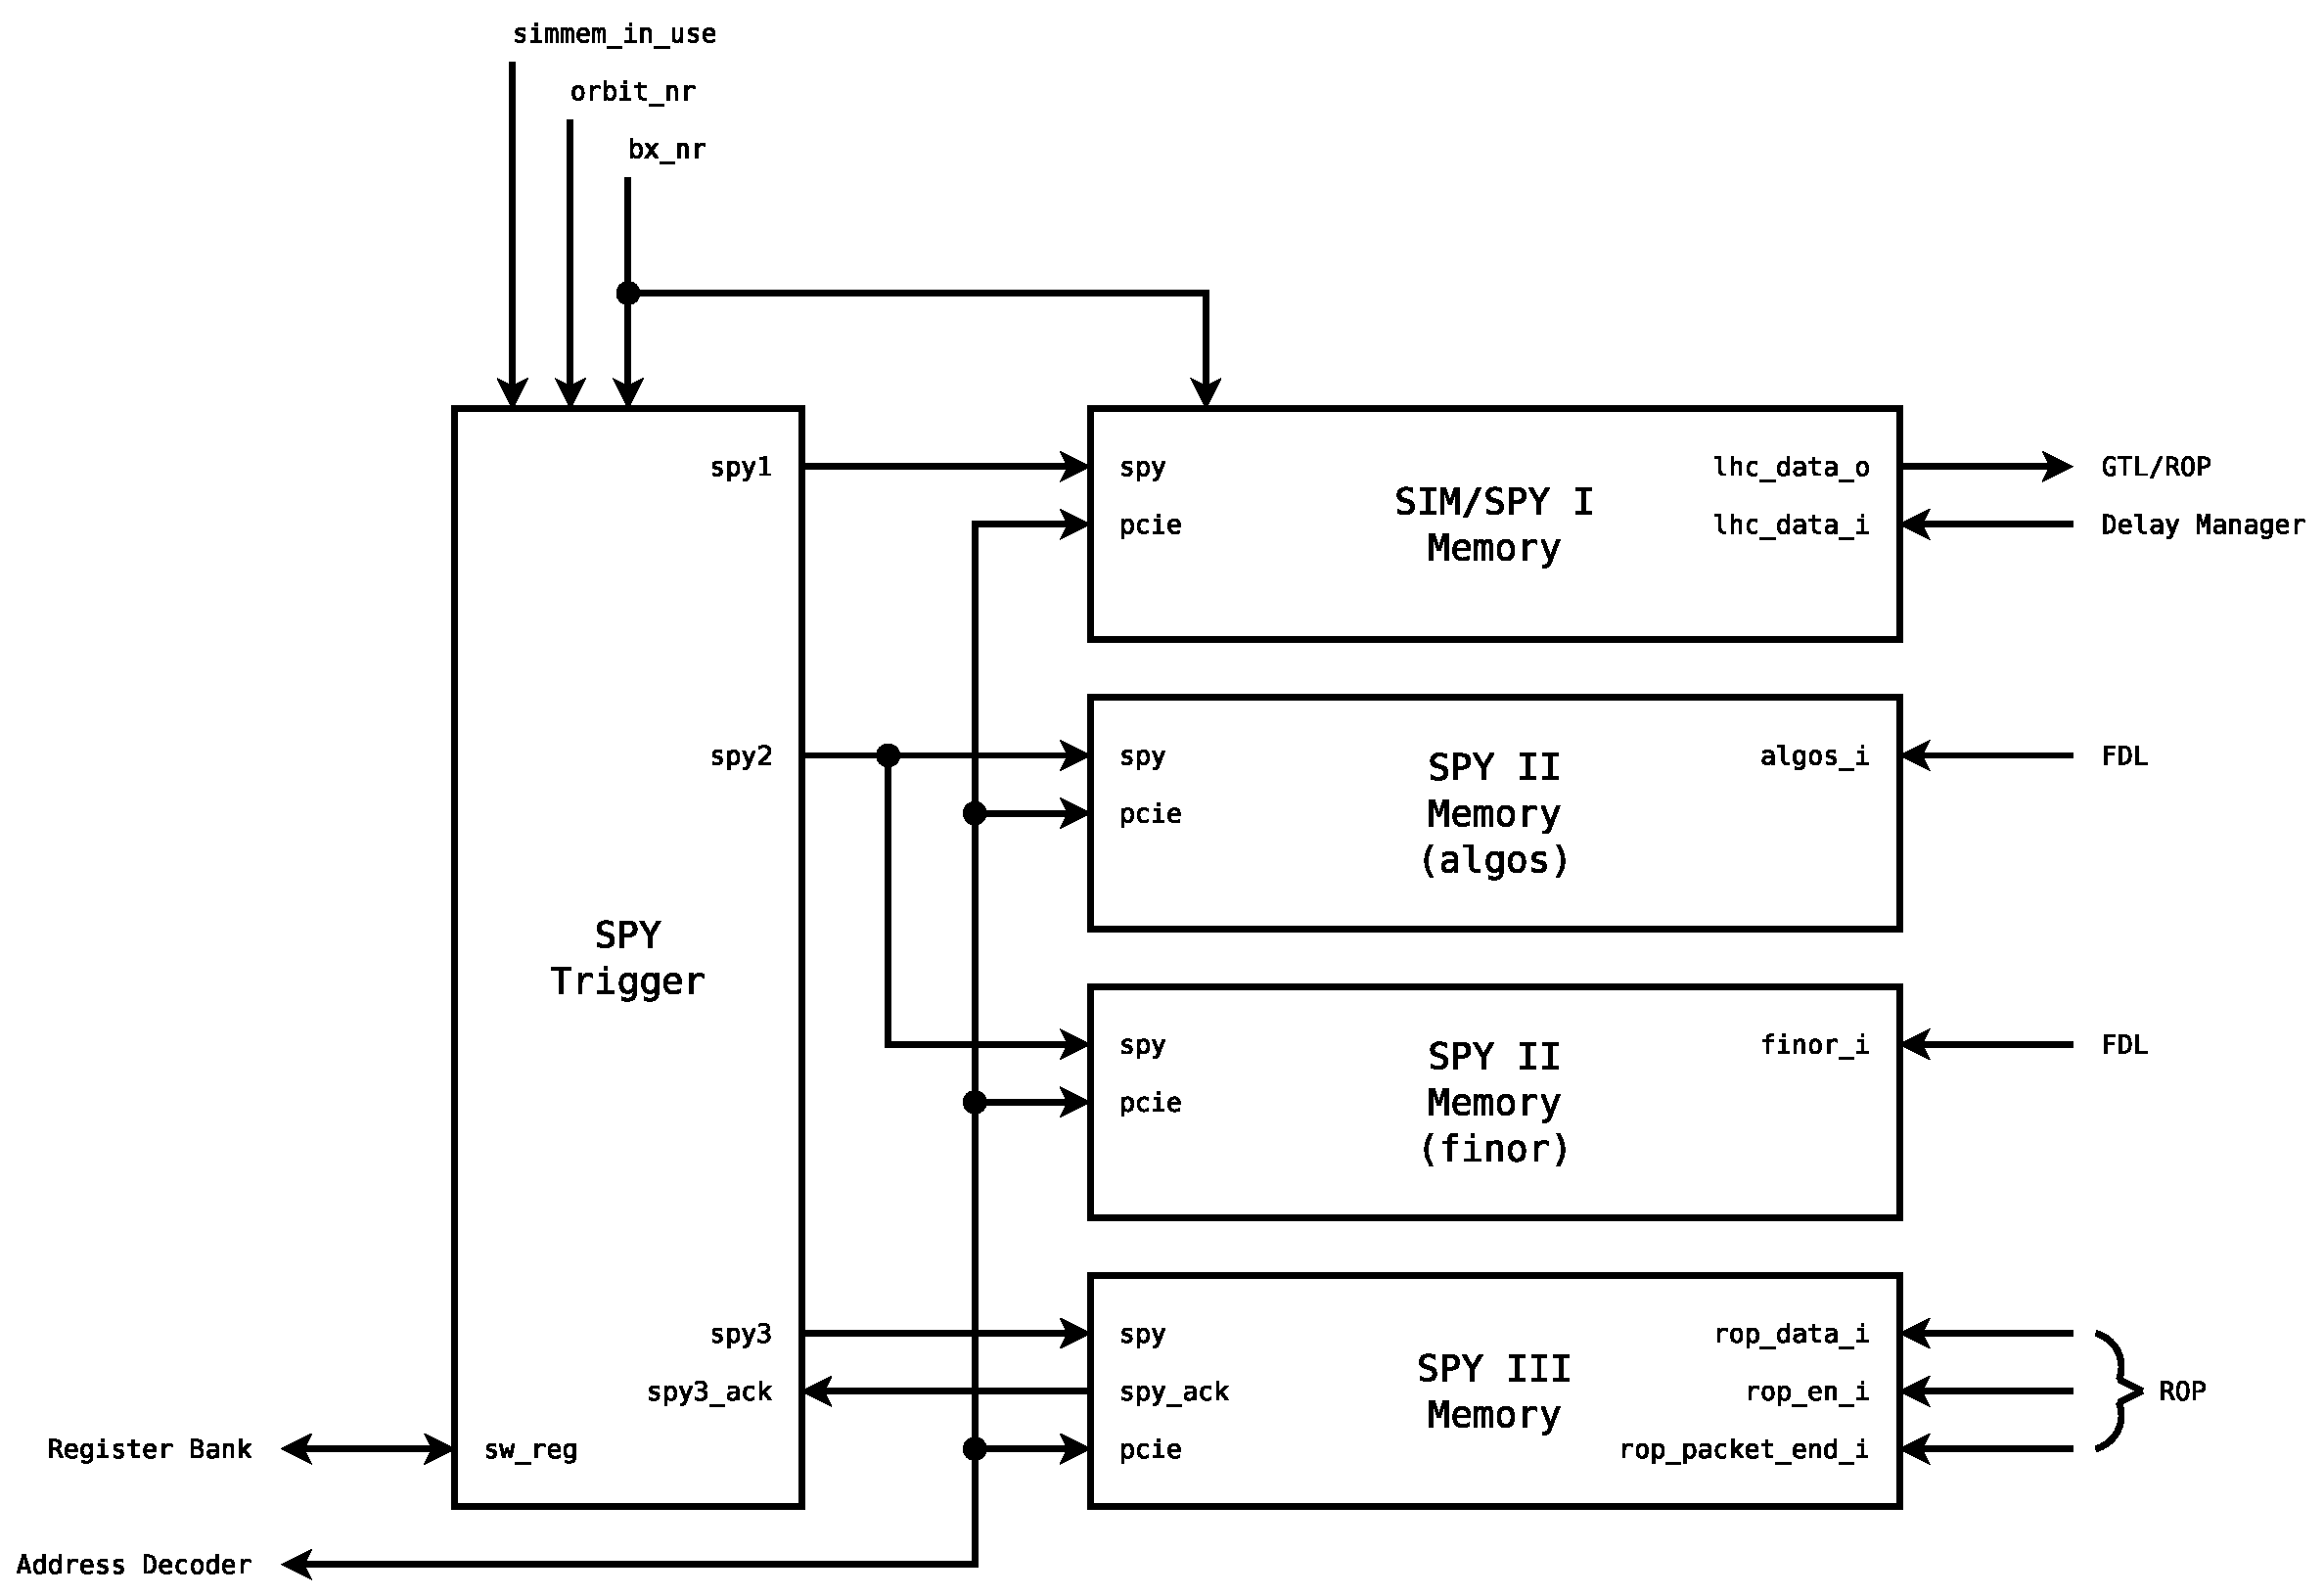
\includegraphics[width=1.0\textwidth]{./figures/simspy}
\caption{Memory subsystem}
\label{fig_simspy}
\end{figure}

\paragraph{SPY Trigger}\label{sec:spy_trigger}
The SPY trigger controls the SPY memories and decides when data is recorded. It can be configured and controlled using 
software registers \ref{spy_trig_obrit_nr_reg} and \ref{spy_trig_cfg_reg} provided by the \hyperref[sec_rb]{register bank}.

\begin{register}{htbp}{SPY Trigger Orbit Number Registers}{}% name=CONFIG
	\label{spy_trig_obrit_nr_reg}
	\regfield{orbit\_nr\_low}{32}{0}{0}%
	\regfield{reserved}{16}{16}{0}%
	\regfield{orbit\_nr\_high}{16}{0}{0}%
	\begin{regdesc}
	\begin{reglist}[Request~Depth]
		\item [orbit\_nr\_low] The 32 low bits of the 48 bit orbit number, used for the spy once trigger.
		\item [orbit\_nr\_high] The 16 high bits of the 48 bit orbit number, used for the spy once trigger.
	\end{reglist}
	\end{regdesc}
\end{register}

\begin{register}{htbp}{SPY Trigger Configuration Register}{}% name=CONFIG
	\label{spy_trig_cfg_reg}%
	\regfield{spy12\_bsy}{1}{31}{0}%
	\regfield{spy3\_bsy}{1}{30}{0}%
	\regfield{spy12\_rdy}{1}{29}{0}%
	\regfield{spy3\_rdy}{1}{28}{0}%
	\regfield{spy12\_err}{1}{27}{0}%
	\regfield{reserved}{21}{6}{0}%
	\regfield{clr\_spy12\_err}{1}{5}{0}%
	\regfield{clr\_spy3\_rdy}{1}{4}{0}%
	\regfield{clr\_spy12\_rdy}{1}{3}{0}%
	\regfield{spy3}{1}{2}{0}%
	\regfield{spy12\_next}{1}{1}{0}%
	\regfield{spy12\_once}{1}{0}{0}%
	\reglabel{Reset}\regnewline%

	\begin{regdesc}
	\begin{reglist}[Request~Depth]
		\item [spy12\_once] Triggers the recording of the selected orbit to SPY memories I and II, when written with 1.
		\item [spy12\_next] Triggers the recording of the next whole orbit to SPY memories I and II, when written with 1.
		\item [spy3] Triggers the recording of the next package that will be sent by the ROP to SPY memory III, when written with 1.
		\item [clr\_spy12\_rdy] Clears the ready flag of the SPY trigger for SPY memories I and II, when written with 1.
		\item [clr\_spy3\_rdy] Clears the ready flag of the SPY trigger for SPY memory III, when written with 1.
		\item [clr\_spy12\_err] Clears the error flag, when written with 1. 
		\item [spy12\_bsy] Indicates that the SPY trigger for SPY memories I and II is busy.
		\item [spy3\_bsy] Indicates that the SPY trigger for SPY memory III is busy.
		\item [spy12\_rdy] Indicates that one orbit has been recorded in SPY memories I and II and that the SPY trigger is ready for new commands.  
		\item [spy3\_rdy] Indicates that packet has been recorded in SPY memory III and that the SPY trigger is ready for new commands. 
		\item [spy12\_err] Indicates an error condition (Set only when the selected orbit number for the spy once trigger lies in the past and can therefore not be recorded).
	\end{reglist}
	\end{regdesc}
\end{register}

When the SPY trigger receives a spy12 command (next or once) over the software register interface it asserts the $spy1$ and $spy2$ signals for the appropriate orbit. 
This means that the $spy$ signals go high with the bunch crossing counter reaching the value zero and stay high until it reaches zero again (overflow). Note that when 
the SIM memory is being used (indicated by the $simem\_in\_use\_i$ input provided by the DSMUX component) the $spy1$ output will not be asserted.

When a spy3 command is received the SPY trigger asserts the $spy3$ signal and waits until the $spy3\_ack$ signal is asserted.

\paragraph{SIM/SPY memory}
This component combines the SIM memory and the SPY memory I. This optimization is possible because these two memories are never used at the same time. There are basically 
two use cases for this memory.
\begin{itemize}
\item SIM memory: Data is read form the memory and provided to GTL and ROP to test these components.
\item SPY memory: External data is received by the GTX and stored in the memory to check the alignment of the data.  
\end{itemize}
It is very important to guarantee that the spy input signal is not asserted, as long as the memory is used as SIM memory. Note that this functionality is implemented in 
the SPY trigger component.

The SIM/SPY memory converts the $lhc\_data\_i$ input signal to a \texttt{std\_logic\_vector} using the converter function provided by the \texttt{lhc\_data\_pkg}. This vector 
is then divided into chunks of 32 bits (the PCIe data width). For each of these chunks a 32 bit true-dual-port memory (2 read ports, 2 write ports, 2 clock domains) is instanciated. 
Thus, every memory has a read/write port in both clock domain, the 125MHz PCIe clock domain and the 40MHz LHC clock domain, which can be used simultaneously.
The PCIe data-in signal ($sw\_i.data$) is connected to PCIe-clock domain write port of the memories. A memory select signal is generated form the LSBs of the software address ($sw\_i.addr$). 
The memory select signal also controls the multiplexer on the output of the memories to generate the $sw\_o.data$ signal.

Depending on whether the SIM/SPY memory is used to provide simulation data or to store/spy data the address on the LHC-clock domain port of the internal memories is adjusted.
If data is recorded (SPY) the bunch crossing counter is used as memory address directly. 
When the memory is read the read latency (two clock cycles) must be taken into account. 
This is achieved by subtracting 2 form the bunch crossing number before using it as address.
To generate the $lhc\_data\_o$ signal the LHC-clock domain data out ports of the internal memories are concatenated and converted back to the \texttt{lhc\_data\_t}.

If the \texttt{lhc\_data\_t} is changed (e.g. new objects added) no modifications in the SIM/SPY memory are required. The SIM/SPY memory only depends on the (auto-generated) 
functions used to convert a \texttt{lhc\_data\_t} signal to \texttt{std\_logic\_vector} and vice versa (see Section \ref{section_lhc_data_pkg} for details).

In the current implementation the size every object in the \texttt{lhc\_data\_t} is a multiple of 32 bit. This is also expected by the SIM/SPY memory. If objects with 16 bit sizes 
are added the SIM/SPY memory must be modified to support this situation (e.g. zero pad the \texttt{lhc\_data\_t}). Furthermore take into account that the PCIe memory bus is 32 bits wide. 
So 16 bit objects should be added to the end of the \texttt{lhc\_data\_t} (as last entry) to keep software memory access simple.

% Table \ref{tab_simpspy} shows the memory layout used to access (read/write) the stored \texttt{lhc\_data\_t}(see Listing \ref{lst_lhc_data_t}). It can be seen that there are areas in 
% the memory that must not be accessed because they do not contain any valid data. 
%require One lhc\_data entry (data for one bunch crossing) needs a memory block 

% \begin{table}[h]
% \begin{center}
% \begin{tabular}{|c|c|}
% \hline
% Address & Data (32 Bit) \\
% (offset from base address) &  \\ \hline
% 0x00000 & BX 0: Muon(0).LOW    \\ \hline
% 0x00001 & BX 0: Muon(0).HIGH   \\ \hline
% 0x00002 & BX 0: Muon(1).LOW    \\ \hline
% 0x00003 & BX 0: Muon(1).HIGH   \\ \hline
% ...    & BX 0: [lhc\_data]    \\ \hline
% 0x00036 & BX 0: External Conditions (7/8) \\ \hline 
% 0x00037 & BX 0: External Conditions (8/8) \\ \hline
% 0x00038 & undefined (do not access) \\ \hline
% ...    & undefined (do not access) \\ \hline
% 0x0003F & undefined (do not access) \\ \hline
% 0x00040 & BX 1: Muon(0).LOW    \\ \hline
% 0x00041 & BX 1: Muon(0).HIGH   \\ \hline
% 0x00042 & BX 1: Muon(1).LOW    \\ \hline
% 0x00043 & BX 1: Muon(1).HIGH   \\ \hline
% ...     & ...       \\ \hline
% 0x37AF7 & BX 3563: External Conditions (8/8)    \\ \hline
% \end{tabular}
% \end{center}
% \caption{SIM/SPY I memory layout}
% \label{tab_simpspy}
% \end{table}
% 
% It is important to note, that the start address of the SIM/SPY memory (configured in the address decoder) must be a multiple of the size of the memory (in the current 
% configuration $2^{18}$ byte addresses).
% To handle/simplify the memory access to this memory special python classes (\verb|GTMemory.py| and \verb|GTMemoryImage.py|) are provided. The XML specification in 
% Listing \ref{lst_lhc_data_t_xml} is used to obtain the memory layout. See the source files for further details and examples of how to use them.

\paragraph{SPY memory II}
The SPY memory II is divided into two subcomponents, to store the $algos$ and $finor$ outputs of the FDL. 
Both memory can only be read over the SW interface. A write access has no effect.
% Tables \ref{tab_spy2_algos} and \ref{tab_spy2_finor} show the memory layout as seen by the software. 
The algos memory uses the same architecture as the SIM memory.
The finor memory uses a true-dual-port memory with asymmetric ports. This memory can be written with a data width of one bit and read with a data width of 32 bit. 

% \begin{table}[h]
% \begin{center}
% \begin{tabular}{|c|c|}
% \hline
% Address & Data (32 Bit) \\
% (offset from base address) &   \\ \hline
% 0x00000 & BX 0: algos: 31-0 (1/16)     \\ \hline
% 0x00001 & BX 0: algos: 64-32 (2/16)    \\ \hline
% ...     & BX 0: ...            \\ \hline
% 0x0000F & BX 0: algos: 511-480 (16/16)   \\ \hline
% 0x00010 & BX 1: algos: 31-0 (1/16)    \\ \hline
% 0x00011 & BX 1: algos: 63-32 (2/16)    \\ \hline
% ...     & BX 1: ...            \\ \hline
% 0x0001F & BX 1: algos: 511-480 (16/16)  \\ \hline
% ...\\ \hline
% 0x0DEBF & BX 3563: algos: 511-480 (16/16)\\ \hline
% \end{tabular}
% \end{center}
% \caption{SPY II algos memory layout}
% \label{tab_spy2_algos}
% \end{table}
% 
% 
% \begin{table}[h]
% \begin{center}
% \begin{tabular}{|c|c|}
% \hline
% Address & Data (32 Bit) \\
% (offset from base address) &   \\ \hline
% 0x00000 & finor for BX 31-0      \\ \hline
% 0x00001 & finor for BX 64-32     \\ \hline
% ...
% 0x00070 & BX 3563: algos: 3552-3563 \\ \hline
% \end{tabular}
% \end{center}
% \caption{SPY II finor memory layout}
% \label{tab_spy2_finor}
% \end{table}
% 
% Note that the start addresses of the algos and finor memories (configured in the address decoder) must be a multiples of their sizes (in the current configuration $2^{16}$ and $2^7$).  
%  
\paragraph{SPY memory III}
The SPY memory III stores the output of the ROP, which is sent to the DAQ. The input data width is configurable to bus widths of 16, 32 or 64 bits.
Depending on the input data width the memory uses different architectures.
\begin{itemize} 
\item 16 Bit \\
A true-dual-port memory with asymmetric ports (16 and 32 bits) is used. 
\item 32 Bit \\
A true-dual-port memory with 32 Bit data width is used.
\item 64 Bit \\
Two true-dual-port memories with 32 Bit data width are used.
\end{itemize}

% \subsubsection{Software}
% The \texttt{gtamc514-memdump} python script can be used to access/read all spy memories of the system.  The \texttt{gtamc514-simmem} script is used to write 
% data to the SIM memory. Refer to See \texttt{gtamc514-memdump -h} and \texttt{gtamc514-simmem -h} for further details.
% 
\subsubsection{Interface Specification}

\begin{minipage}{\textwidth}
\lstinputlisting[language=VHDL,caption=SPY trigger interface specification]{interfaces/spytrig.vhd}
\end{minipage}

% \begin{minipage}{\textwidth}
% \lstinputlisting[language=VHDL,label=lst_simspymem,caption=SIM/SPY I memory interface specification]{interfaces/simspymem.vhd}
% \end{minipage}
% 
% \begin{minipage}{\textwidth}
% \lstinputlisting[language=VHDL,caption=SPY memory II (algos) interface specification]{interfaces/spymem2_algos.vhd}
% \end{minipage}
% 
% \begin{minipage}{\textwidth}
% \lstinputlisting[language=VHDL,caption=SPY memory II (finor) interface specification]{interfaces/spymem2_finor.vhd}
% \end{minipage}
% 
% \begin{minipage}{\textwidth}
% \lstinputlisting[language=VHDL,caption=SPY memory III interface specification]{interfaces/spymem3.vhd}
% \end{minipage}
% 
%------------------------------------------------------------------------------
%
%  L1A Simulator
%
% ------------------------------------------------------------------------------
% \subsection{L1A Simulator}
% 
% The simulation component for the l1a signal has been reimplemented based on specification of the last semester.
% 
% The L1A SIM/MUX module takes as input the synchronized real l1a signal (usually originating from the TCS) and outputs depending on its configuration the (undelayed) real l1a signal or a simulation of the signal. The following simulation modes which are configurable through software register access are available:
% \begin{itemize}
% \item fire once: the l1a signal is set to high for exactly one clock cycle as soon as the software
% register access has been issued. Note that this mode overrides both, the real l1a and
% any simulation mode. After the single l1a event completed, the L1A SIM/MUX module
% continues operation according to the sim\_mode register.
% \item pattern at orbit: replay a predefined l1a pattern at a specified orbit counter value.
% \item alternating patterns: replay a predefined l1a pattern at an even orbit counter value,
% followed by another predefined l1a pattern at an odd orbit counter value. This mode
% is freerunning: the two orbit patterns are replayed in an alternating way as long as the
% mode is active.
% \end{itemize}
% A l1a pattern consists of bunch crossing number (bx\_nr) compare values that indicate
% when exactly the simulated l1a signal is supposed to be active (set to high). As the maximum
% frequency of l1a signal occurrences is 100 kHz (10 l1a events per orbit), a l1a pattern
% consists of 10 such bunch crossing counter compare values. Not all of the 10 places need to be
% used: in case a bunch crossing counter compare value is higher than BUNCHES\_PER\_ORBIT-1
% (e.g. 0xdec), but lower than 0x1000, it is ignored. Alternatively unused places can also be
% set to values that are already specified.
% Through software register access 2 l1a pattern can be specified: pattern A and pattern B. For
% the first mode (fire once) no pattern is considered, for the second mode (pattern at orbit), only
% pattern A is used and for the last mode (alternating patterns), pattern A (even orbits) and
% pattern B (odd orbits) are used. In case both, the second and the third mode are activated
% by software register access, the third mode overrides the second one.
%  
% Registers \ref{l1asim_cfg_reg} \ref{l1asim_orbit_nr_reg} \ref{l1asim_pattern_reg} specify the software interface.
% 
% \begin{register}{htbp}{L1A Simulator Configuration Register}{}% name=CONFIG
% 	\label{l1asim_cfg_reg}%
% 	\regfield{reserved}{28}{4}{0}%
% 	\regfield{sim\_mode}{2}{2}{0}%
% 	\regfield{fire\_once}{1}{1}{0}%
% 	\regfield{enable\_sim}{1}{0}{0}%
% 	\reglabel{Reset}\regnewline%
% 
% 	\begin{regdesc}
% 	\begin{reglist}[Request~Depth]
% 			\item [enable\_sim] Enables the l1a simulation module. This bit must be 1 for all other configurations to have an effect. If this bit is zero the real l1a signal is presented at the output of the l1asim module.
% 			\item [fire\_once] When written with 1, triggers one l1a event as soon as the hardware recognizes the register access (It is not possible to exactly time the event using this trigger)
% 			\item [sim\_mode] Selects one of the two simulation modes (pattern at orbit, alternating patterns). If zero (00) no mode is selected. 
% 	\end{reglist}
% 	\end{regdesc}
% \end{register}
% 
% \begin{register}{htbp}{L1A Simulator Orbit Number Registers}{}% name=CONFIG
% 	\label{l1asim_orbit_nr_reg}
% 	\regfield{orbit\_nr\_low}{32}{0}{0}%
% 	\regfield{reserved}{16}{16}{0}%
% 	\regfield{orbit\_nr\_high}{16}{0}{0}%
% 	\begin{regdesc}
% 	\begin{reglist}[Request~Depth]
% 		\item [orbit\_nr\_low] The 32 low bits of the 48 bit orbit number, used for the pattern at orbit simulation mode.
% 		\item [orbit\_nr\_high] The 16 high bits of the 48 bit orbit number, used for the pattern at orbit simulation mode.
% 	\end{reglist}
% 	\end{regdesc}
% \end{register}
% 
% \begin{register}{htbp}{L1A Simulator Pattern Registers}{}% name=CONFIG
% 	\label{l1asim_pattern_reg}
% 	\regfield{reserved}{20}{12}{0}%
% 	\regfield{bx\_nr}{12}{0}{0}%
% 	\begin{regdesc}
% 	\begin{reglist}[Request~Depth]
% 		\item [bx\_nr] The 12 bit bunch crossing number, used for the pattern at orbit and the alternating patterns simulation mode. Currently there are 10 pattern registers available (l1asim\_pattern\_a[0-4] and l1asim\_pattern\_b[0-4])
% 	\end{reglist}
% 	\end{regdesc}
% \end{register}
% 
% \subsubsection{Interface Specification}
% 
% \begin{minipage}{\textwidth}
% \lstinputlisting[language=VHDL,caption=L1A Simulation module interface specification]{interfaces/l1asim.vhd}
% \end{minipage}
% 
%------------------------------------------------------------------------------
%
%  TCM
%
% ------------------------------------------------------------------------------
\subsection{TCM}\label{sec:tcm}
\textbf{\textit{Under construction!!!}}

The Timer Counter Manager (TCM) provides different counters, listed in table \ref{tab:tcm_counters}.

\subsubsection{Counter Overview}
\begin{table}[H]
\vspace{5mm}
\begin{scriptsize}
\begin{tabular}{|l|l|l|l|l|}
\hline
Counter             &range              &increase condition               &reset condition           &Comments     \\ \hline
bx\_nr              &$0 to 3563$        &rising\_edge(lhc\_clk)           &overflow                  &             \\ \hline
event\_nr           &$0 to 2^{32}-1$    &l1a=1 and rising\_edge(lhc\_clk) &BGOS: event counter reset &             \\ \hline
trigger\_nr         &$0 to 2^{48}-1$    &l1a=1 and rising\_edge(lhc\_clk) &BGOS: start run           &             \\ \hline
orbit\_nr           &$0 to 2^{48}-1$    &overflow of bx\_nr               &BGOS: orbit counter reset &             \\ \hline
luminosity\_seg\_nr &$0 to 2^{32}-1$    &rising\_edge(orbit\_nr(18))      &BGOS: orbit counter reset &             \\ \hline
start\_lumisection  &$0 to 1$           &luminosity\_seg\_nr increases    &after 25ns                &'1' for 25ns \\ \hline
bx\_nr\_d\_fdl      &$0 to 3563$       &rising\_edge(lhc\_clk)            &overflow                  &             \\ \hline
\end{tabular}\caption{counters of the timer counter manager}\label{tab:tcm_counters}
\end{scriptsize}
\end{table}

\subsubsection{Bunch Crossing Number and counters derived from it}
All counters except for event\_nr and the trigger\_nr (which are trivial because they are increased with l1a) are dependent on the bunch crossing counter bx\_nr as stated in table \ref{tab:tcm_counters}. The bx\_nr is zero at startup, then waits for the the first bcres\_d (bunch crossing reset delayed) and starts counting as depicted in figure \ref{fig:bx_start}. It's maximal value is 3563 (0xdeb), then it automatically overflows and starts at zero again (see figure \ref{fig:bx_normal_operation}). Exactly when bx\_nr = 0, bcres\_d has to be asserted. Otherwise the counter is out of synchronization. If this happens, the software register err\_det is set and the counter waits for the next bcres\_d to synchronize again. Note that the value of the counter is invalid until it has synchronized again.

\begin{figure}[ht]
  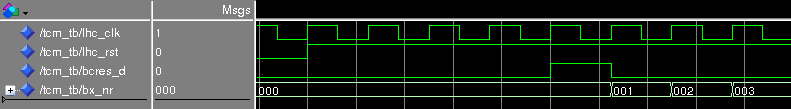
\includegraphics[width=1.0\textwidth]{./figures/bx_start}
  \caption{start of the bunch crossing number with the first bcres\_d}
  \label{fig:bx_start}
\end{figure}

\begin{figure}[ht]
  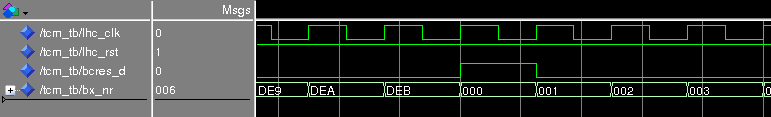
\includegraphics[width=1.0\textwidth]{./figures/bx_normal_operation}
  \caption{normal operation of the bunch crossing number}
  \label{fig:bx_normal_operation}
\end{figure}

\subsubsection{Special counter: bx\_nr\_d\_fdl}
The bx\_nr\_d\_fdl is derived from bcres\_d\_fdl in the same manner as bx\_nr is derived from bcres\_d. bx\_nr\_d\_fdl will automatically resync if the logic described in subsection \ref{subsec:tcmerrors} detects a synchronization error for bx\_nr.

\subsubsection{Counters derived from l1a}
The counters event\_nr and trigger\_nr are increased with l1a, i.e. they are increased twice if l1a is high for 2 clock cycles, etc. They differ only in their value range and the condition that resets the counters, see table \ref{tab:tcm_counters}.

\subsubsection{Errors}\label{subsec:tcmerrors}
As stated above, bcres\_d has to be asserted exactly when bx\_nr = 0, otherwise the counter is out of sync. Then the software register err\_det is set as depicted in figure \ref{fig:err_det}. err\_det can be reset via the software event register err\_det\_reset\_event as depicted in figure \ref{fig:err_det_reset}. Furthermore err\_det is set if bgos = Resync-0x1 and the counter value is not 3563.

\begin{figure}[ht]
  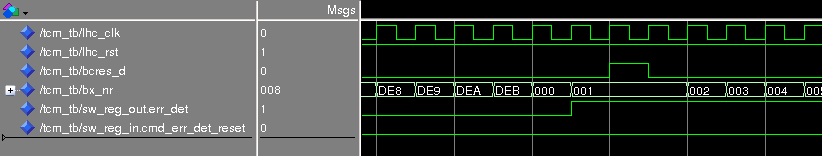
\includegraphics[width=1.0\textwidth]{./figures/err_det}
  \caption{set of the software register err\_det when bc\_res\_d is not asserted correctly}
  \label{fig:err_det}
\end{figure}

\begin{figure}[ht]
  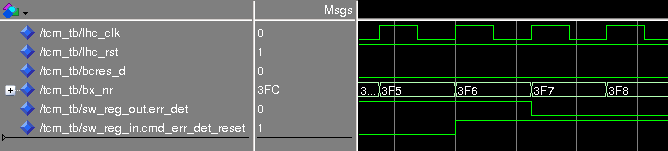
\includegraphics[width=1.0\textwidth]{./figures/err_det_reset}
  \caption{reset of the software register err\_det when err\_det\_reset\_event toggles}
  \label{fig:err_det_reset}
\end{figure}

The TCM implements two additional counters (bx\_nr\_chk and bx\_nr\_max) for debugging purposes. These counters are not visible by any other module but readable via software. bx\_nr\_chk is a 32bit Counter that increases with every LHC clock cycle and resets with bcres\_d. bx\_r\_max holds the highest value bx\_nr\_chk ever reached (should be 3563 if the link is aligned).

\subsubsection{SW-Registers}
All counters except for the start\_lumisection described in table \ref{tab:tcm_counters} can be read by software via the following sw registers:

\begin{register}{H}{TCM Bunch Crossing Number Register}{}%
	\regfield{reserved}{20}{12}{0}%
	\regfield{bx\_nr}{12}{0}{0}%
	\begin{regdesc}
	\end{regdesc}
\end{register}
\begin{register}{H}{TCM Event Number Register}{}%
	\regfield{event\_nr}{32}{0}{0}%
	\begin{regdesc}
	\end{regdesc}
\end{register}
\begin{register}{H}{TCM Trigger Number Registers}{}%
	\regfield{trigger\_nr\_l}{32}{0}{0}%
	\regfield{reserved}{16}{16}{0}%
	\regfield{trigger\_nr\_h}{16}{0}{0}%
	\begin{regdesc}
	\begin{reglist}[Request~Depth]
		\item [trigger\_nr\_l] The 32 low bits of the 48 bit trigger number.
		\item [trigger\_nr\_h] The 16 high bits of the 48 bit trigger number.
	\end{reglist}
	\end{regdesc}
\end{register}
\begin{register}{H}{TCM Orbit Number Registers}{}%
	\regfield{orbit\_nr\_l}{32}{0}{0}%
	\regfield{reserved}{16}{16}{0}%
	\regfield{orbit\_nr\_h}{16}{0}{0}%
	\begin{regdesc}
	\begin{reglist}[Request~Depth]
		\item [orbit\_nr\_l] The 32 low bits of the 48 bit orbit number.
		\item [orbit\_nr\_h] The 16 high bits of the 48 bit orbit number.
	\end{reglist}
	\end{regdesc}
\end{register}
\begin{register}{H}{TCM Luminosity Segment Number Register}{}%
	\regfield{luminosity\_seg\_nr}{32}{0}{0}%
	\begin{regdesc}
	\end{regdesc}
\end{register}
\begin{register}{H}{TCM Bunch Crossing Number FDL Register}{}%
	\regfield{reserved}{20}{12}{0}%
	\regfield{bx\_nr\_d\_fdl}{12}{0}{0}%
	\begin{regdesc}
	\end{regdesc}
\end{register}
\begin{register}{H}{TCM Bunch Crossing Number Check Register}{}%
	\regfield{bx\_nr\_chk}{32}{0}{0}%
	\begin{regdesc}
	\end{regdesc}
\end{register}
\begin{register}{H}{TCM Bunch Crossing Number Max Register}{}%
	\regfield{bx\_nr\_max}{32}{0}{0}%
	\begin{regdesc}
	\end{regdesc}
\end{register}

Some additional control register can be used to check and reset err\_det, disable the check of bcres\_d and bcres\_d\_fdl (bx\_nr and bx\_nr\_d\_fdl automatically reset when they overflow if cmd\_ign\_bcres is set, bcres\_d is ignored) and simulate the bgos signal. To do this, a value of the orbit signal has to be written to sw-register bgos. The value of the input signal bgos is replaced by the value of the sw-register for exactly one clock cycle, when "1" is written to the event register bgos\_event.

\begin{register}{H}{TCM cmd\_ign\_bcres}{}% name=CONFIG
	\label{cmd_ign_bcres}%
 	\regfield{reserved}{31}{1}{0}%
 	\regfield{cmd\_ign\_bcres}{1}{0}{0}%
	\reglabel{Reset}\regnewline%

	\begin{regdesc}
	\begin{reglist}[Request~Depth]
 		\item [cmd\_ign\_bcres] bcres is ignored (not checked) when this is set.
	\end{reglist}
	\end{regdesc}
\end{register}

\begin{register}{H}{TCM err\_det}{}% name=CONFIG
	\label{err_det}%
 	\regfield{reserved}{31}{1}{0}%
	\regfield{err\_det}{1}{0}{0}%
	\reglabel{Reset}\regnewline%

	\begin{regdesc}
	\begin{reglist}[Request~Depth]
		\item [err\_det] Set when out of synchronization.
	\end{reglist}
	\end{regdesc}
\end{register}

\begin{register}{H}{TCM err\_det\_reset\_event}{}% name=CONFIG
	\label{err_det_reset_event}%
 	\regfield{reserved}{31}{1}{0}%
 	\regfield{err\_det\_reset\_event}{1}{0}{0}%
	\reglabel{Reset}\regnewline%

	\begin{regdesc}
	\begin{reglist}[Request~Depth]
 		\item [err\_det\_reset\_event] Event register: resets err\_det.
	\end{reglist}
	\end{regdesc}
\end{register}

\begin{register}{H}{TCM bgos}{}% name=CONFIG
	\label{bgos}%
 	\regfield{reserved}{31}{4}{0}%
 	\regfield{bgos}{4}{0}{0}%
	\reglabel{Reset}\regnewline%

	\begin{regdesc}
	\begin{reglist}[Request~Depth]
 		\item [bgos] For simulation of the bgos signal.
	\end{reglist}
	\end{regdesc}
\end{register}

\begin{register}{H}{TCM bgos\_event}{}% name=CONFIG
	\label{bgos_event}%
 	\regfield{reserved}{31}{1}{0}%
 	\regfield{bgos\_event}{1}{0}{0}%
	\reglabel{Reset}\regnewline%

	\begin{regdesc}
	\begin{reglist}[Request~Depth]
 		\item [bgos\_event] Event register: replaces the input signal bgos by the sw-register bgos for exactly one clock cycle.
	\end{reglist}
	\end{regdesc}
\end{register}

\begin{register}{H}{TCM luminosity\_seg\_period\_msk}{}% name=CONFIG
	\label{luminosity_seg_period_msk}%
 	\regfield{luminosity\_seg\_period\_msk}{32}{0}{0x40000}%
	\reglabel{Reset} %\regnewline%

	\begin{regdesc}
	\begin{reglist}[Request~Depth]
 		\item [luminosity\_seg\_period\_msk] luminosity\_seg\_nr is increased when the orbit\_nr mod lum\_seg\_period\_mask = 0.
	\end{reglist}
	\end{regdesc}
\end{register}

\subsubsection{Hardware Test}
There are various python scripts located in the software/GtControl/branches/fpga-design-2013/python/GtControl directory for testing the tcm module. Please refer to the output of the scripts for information how the tests are performed in detail. See table \ref{tab:tcm_hw_test}.
\begin{table}[ht]
\vspace{5mm}
\begin{scriptsize}
\begin{tabular}{|p{5cm}|p{10cm}|}
\hline
script                         &purpose    \\ \hline
\verb|tcm_counter_values.py|   &outputs the values of all counters defined above    \\ \hline
\verb|tcm_produce_err_det|     &produces an err\_det by manipulating bgos \\ \hline
\verb|tcm_err_det_reset|       &resets the err\_det software register \\ \hline
\verb|tcm_trigger_test|        &tests trigger\_nr and event\_nr by generating l1a signals using l1asim \\ \hline
\verb|tcm_lum_seg_nr_test|    &checks the period of two successive increases of the luminositiy\_seg\_nr \\ \hline
\end{tabular}\caption{scripts for testing the tcm}\label{tab:tcm_hw_test}
\end{scriptsize}
\end{table}

% \subsubsection{Interface}
% 
% \lstinputlisting[language=VHDL,caption=TCM interface specification]{interfaces/tcm.vhd} 

\subsection{Software Reset} \label{sec:software_reset}
The software reset module (sw\_reset) provides the possiblity for a software reset via the software event register sw\_reset\_event.

\begin{register}{htbp}{Software Reset register}{}% name=CONFIG
	\label{tcm_ctrl_reg}%
	\regfield{reserved}{31}{1}{0}%
	\regfield{sw\_reset\_event}{1}{0}{0}%
	\reglabel{Reset}\regnewline%

	\begin{regdesc}
	\begin{reglist}[Request~Depth]
		\item [sw\_reset\_event] Event register: Generates a reset signal for exactly one clock cycle.
	\end{reglist}
	\end{regdesc}
\end{register}

\clearpage






